\documentclass[UTF8]{ctexart}

\usepackage{subfiles}  

%下面的语句, 引入你的头部设置文件
\usepackage{C:/phpStorm_proj/02_myself_ID_EGO/+100_latex_all_math_sel/myPreamble} 
%必须是绝对路径,才能让各个tex在单独编译时使用到

\title{物理}


%---------------------------------


\begin{document}
	\tableofcontents % 生成目录
	\date{} % 若不写这句, 则默认也会渲染出日期, 所以我们要手动赋空值
	\maketitle  %这行代码, 让你前面的 title, author, date生效
	
	
	\section{摆的等时性}
	
	摆的等时性 : 无论摆动的幅度大还是小, 完成一次摆动的时间是一样的.	
	
	各种机械摆钟, 就是根据这个原理制作的.
	
	摆绳越长, 往复摆动一次的时间(即周期), 也就越长.
	
	
~\\
\hrule
~\\
	
	
	
	\section{质量 mass}
	
	\textbf{质量: 物体所含物质的多少, 叫做``质量" mass.} 公式中就用其首字母 m 来表示. \\
	
	质量的单位是:	 \\
	- 1 t 吨 = 1000 kg \\
	- 1 kg 千克(即公斤) \\
	- 1 g 克 = 1000 mg \\
	- 1 mg 毫克 \\
	
	地球的质量 = $ 5.97237 \cdot 10^{24} \ kg $ \\
	太阳的质量 = $ 1.9891 \cdot 10^{30} \ kg $ \\
	
	称质量的工具: 秤  \\
	
	\textbf{质量无关``物态": 一块冰融化成水, 其质量不会改变.} \\	
	质量也无关``所处的位置": 一个东西在地球上, 或带到太空里, 其质量不会改变. \\
	即: 物体的质量, 不随它的物态, 位置而改变. 
	
	
	~\\
	\hrule
	~\\
	
	
	\section{$\text{密度}\rho =\frac{\text{质量}m}{\text{体积}V}$}
	
	同一种物体, 体积越大, 质量越大. \\
	密度 density : 由某种物质组成的物体的``质量", 与它``体积"之比, 就是这种物体的``密度". 
	
	\begin{align*}
		\boxed{
			\text{密度}\rho =\dfrac{\text{质量}m}{\text{体积}V}
		}
	\end{align*}

	这个公式就是说: \textbf{``密度"在数值上, 等于``物体单位体积的质量".} \\

	密度ρ的单位, 是由``质量的单位" 和 ``体积的单位" 共同组成的. 即, \textbf{密度的基本单位就是: $ kg/m^3$ (千克/立方米), 或 $ g/cm^3$ (克/立方厘米).} \\

	这两个密度单位的关系是: 
	\begin{align*}
		\boxed{			
		1 g / cm^3 = 1 \cdot 10^3 kg/m^3
		}
	\end{align*}
	1 克/立方厘米(克每立方厘米) = 1000 千克/立方米(千克每立方米) \\
	
	
	
	~\\
	\hrule
	~\\
	
	
	
	\section{大气压强}
	
	\subsection{标准大气压强 :  $1.013\cdot 10^5\ P_a$}
	
	大气压强, 简称为大气压(atmosphere), 或气压。\textbf{注意:大气压是"大气压强"的简称,不是"大气压力"的简称.} \\
	
	大气压产生的原因: 由于大气受到重力的作用而产生. \\
	大气压的方向: 同液体一样, 大气朝向各个方向都有压强的. \\
	
	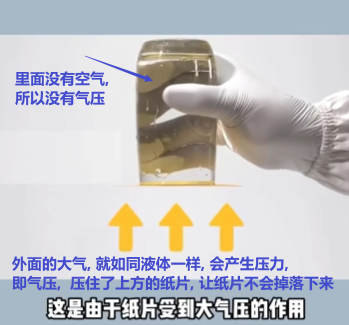
\includegraphics[width=0.3\textwidth]{img/0024.png}
	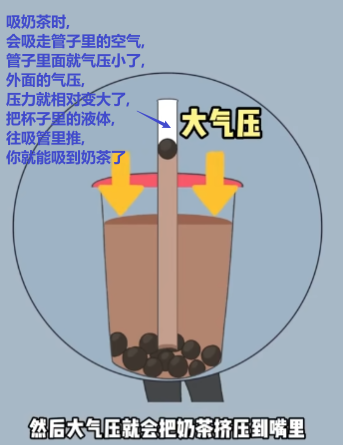
\includegraphics[width=0.3\textwidth]{img/0025.png}
	
	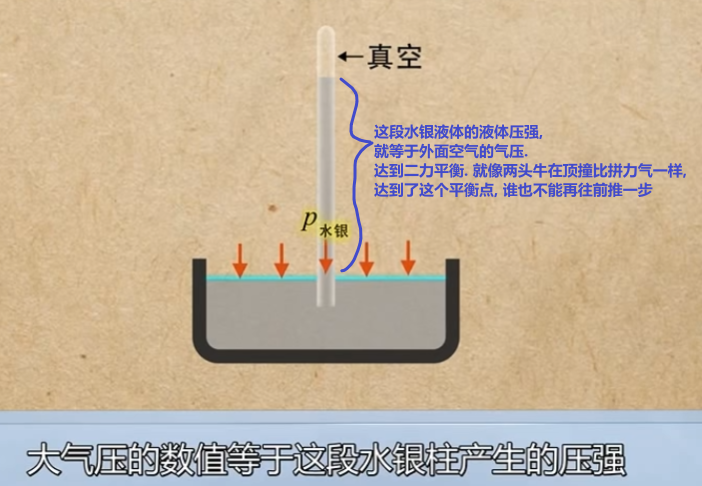
\includegraphics[width=0.3\textwidth]{img/0026.png}	
	
\includegraphics[width=0.3\textwidth]{img/0028.png}
	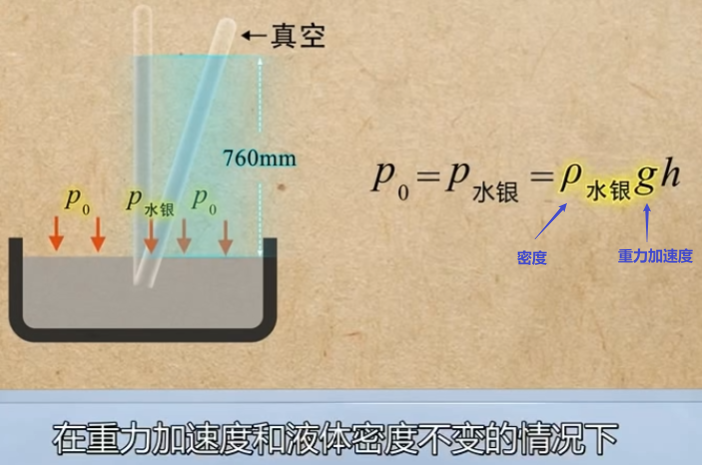
\includegraphics[width=0.3\textwidth]{img/0029.png} \\
	
	水银柱产生的压强 $p_{\text{水银}}=\text{标准大气压}p_0$, 根据压强公式 p=ρgh, 在水银密度ρ不变, 重力加速度g=9.8N/kg, 标准大气压 $p_0$,  这三个变量都不变的情况下, 显然水银柱的高度h 就不会改变.
	
	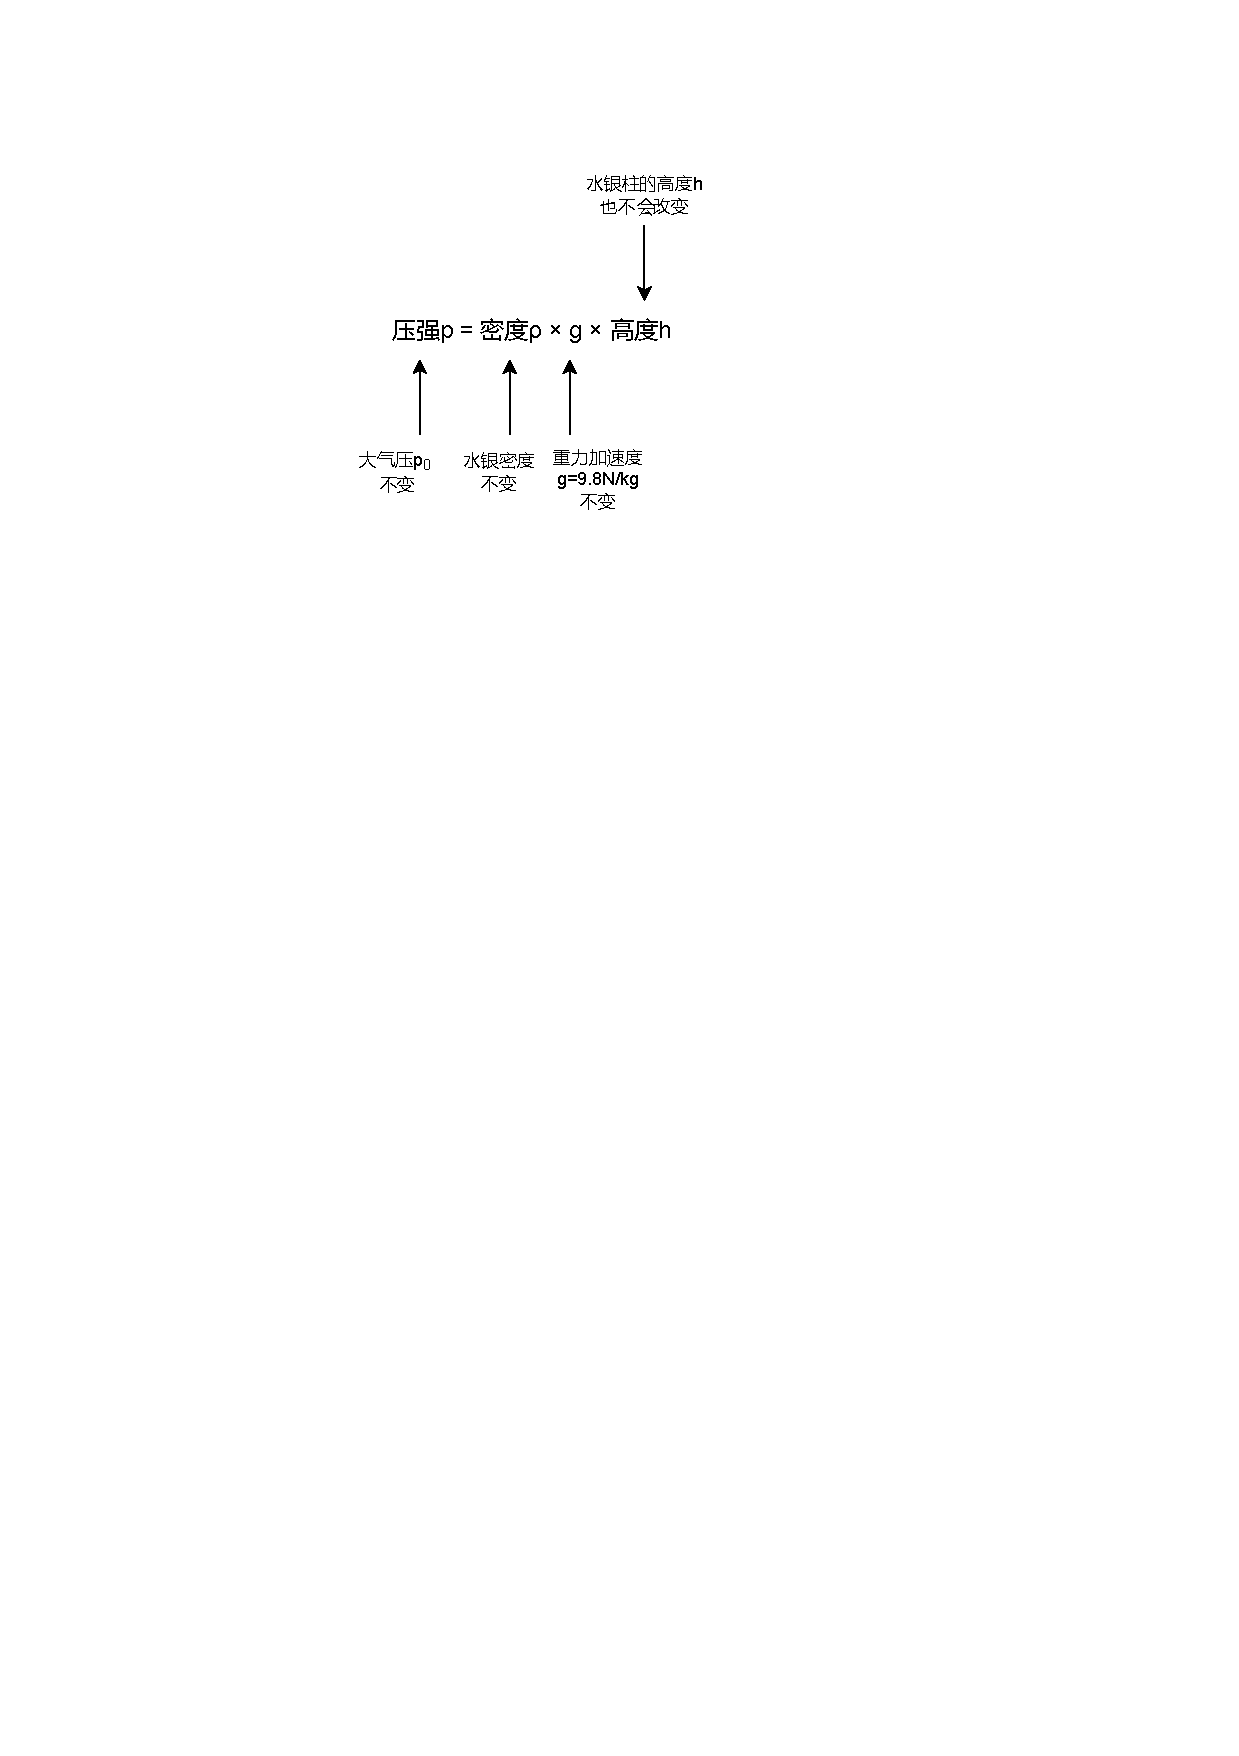
\includegraphics[width=0.3\textwidth]{img/0031.pdf} 
	
	同时这也说明, 某液体或气体深处的压力的大小, 跟其质量m的多少无关. 即使水银柱倾斜过来, 水银柱中水银的体积增加, 质量m增加, 它的压强p也不会改变. \\
	
	注意:只有在水银柱上部的空间是``真空"时, 水银柱的压强才跟大气压强相等. 如果水银柱上方不是真空, 而是混有空气, 则这段空间的气体, 也会对水银柱产生压强. 在这种情况下, 就是这个压强与水银柱产生的压强之和, 才等于大气压强.
	
	即: 管内水银柱的高度, 只随外界大气压的变化而变化, 而和管子的粗细、倾斜角度、管的长度, 及将玻璃管提起还是下压等因素无关. 只与水银柱的竖直高度有关. \\
	
	注意: 大气的密度是变化的, 在地面附近, 空气的密度较大, 随高度的增加, 空气的密度越来越小. \\
	
	所以, \textbf{在地表的大气压下, 压得水银柱高度为760 mm. 反过来说, 我们就把这样大小的大气压, 叫做``标准大气压" $p_0$.}
	
	\begin{align*}
		\boxed{
			\underset{\text{标准大气压}}{\underbrace{p_0}}=\underset{\text{水银密度}13.59g/cm³}{\underbrace{\rho }}\cdot \underset{9.8N/kg}{\underbrace{g}}\cdot \underset{0.76m}{\underbrace{h}}=1.013\cdot 10^5\ P_a			
		}
	\end{align*}
	
	水银的密度, 是水的密度的13.6倍. 
	
	\textbf{在粗略计算中, 标准大气压可以取为 $1×10^5 Pa$.}
		
	\vspace{1em} 
	
	
	
	\subsection{``标准大气压"下的水柱的高度是 10.336米}
	
	如果玻璃管中装的是水呢?	
	\begin{align*}  % 支持每行编号. 若不需要编号, 就用 align*环境
	& \underset{\text{标准大气压}}{\underbrace{p_0}}=p_{\text{水银}}=p_{\text{水}}\\
	& \text{即:\ }\underset{\text{水银密度}13.59g/cm³}{\underbrace{\rho }}\cdot \underset{9.8N/kg}{\underbrace{g}}\cdot \underset{0.76m}{\underbrace{h}}=\underset{\text{水的密度1.0\ }kg/m³}{\underbrace{\rho }}\cdot \underset{9.8N/kg}{\underbrace{g}}\cdot \underset{\text{水柱的高度}}{\underbrace{h}}\\
	& \text{最终会得到\ }h_{\text{水}}=10.336m\\ 
	\end{align*}
		
	\vspace{1em} 
	
	
	
	\subsection{(1)高度越高, 空气密度越小, 气压就越低. (2)气压越低, 沸点也就越低}
	
	从气压公式也可知道: \textbf{随着高度的升高(即 深度h 的减少. 你只需把空气想象成大海, 越接近地表的空气, 就如同海底的深度一样, 深度最大. 即 h最大. 这样, 随着海拔的增加, 越往天上去, 空气的深度h就越小, 气压就越小).}  换种说法就是: 海拔升高,空气就越稀薄,密度越小,所以大气压会减小. 瓶中的空气的气压值超过了外面的气压, 就会将瓶中的水挤压到玻璃管中,  水柱的高度就会逐渐升高。
	
	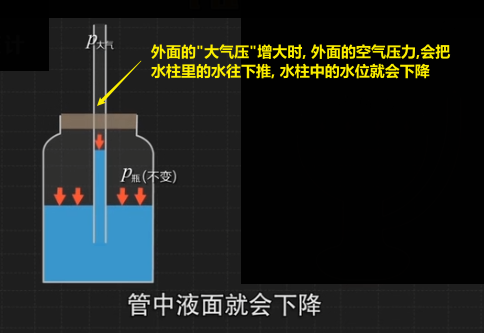
\includegraphics[width=0.45\textwidth]{img/0032.png} 
	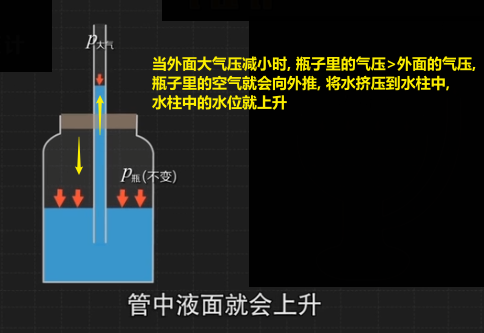
\includegraphics[width=0.45\textwidth]{img/0033.png} 
	
	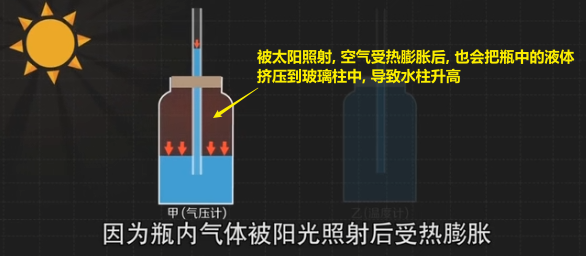
\includegraphics[width=0.45\textwidth]{img/0036.png} 	
	
	在海拔3000m 以内, 大约每升高10m, 大气压减小100 Pa. \\
	
	液体的沸点跟外部压强有关。当液体所受的压强(比如气压)增大时, 沸点也升高; 压强减小时,沸点也降低.   \\	
	- 蒸汽锅炉里的蒸汽压强,约有几十个大气压,锅炉里的水的沸点可在200℃以上. \\	
	- 在高山上煮饭,比如青藏高原, 水的沸点仅为 84-87℃, 水就沸腾了,但饭不易熟. 所以必须使用压力锅做饭, 以增强压力, 让沸点升高.
	
	
	
	
	
	
	
	\vspace{1em} 
	
	\subsection{自制气压计: 瓶中必须存在空气, 才能有气压, 才能在瓶中内外造成气压差.}
	
	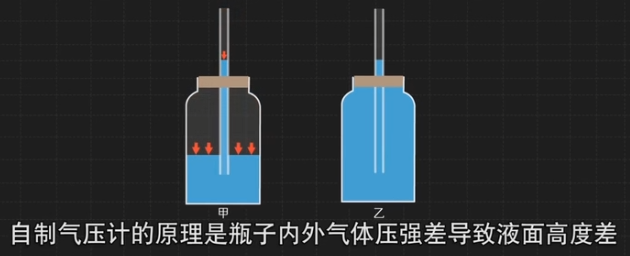
\includegraphics[width=0.45\textwidth]{img/0034.png} 
	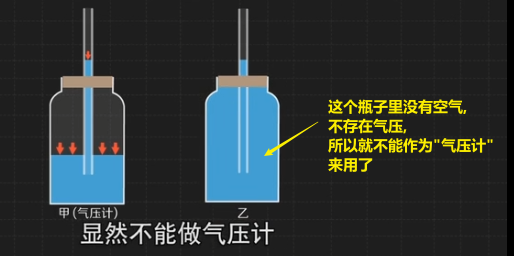
\includegraphics[width=0.45\textwidth]{img/0035.png} 
	
	
	
	
	~\\
	\hrule
	~\\
	
	
	
	45
	
	
	
	
\end{document}